\documentclass{article}
\usepackage{arxiv}

\usepackage[utf8]{inputenc}
\usepackage[english, russian]{babel}
\usepackage[T1]{fontenc}
\usepackage{url}
\usepackage{booktabs}
\usepackage{amsfonts}
\usepackage{bbm}
\usepackage{nicefrac}
\usepackage{microtype}
\usepackage{lipsum}
\usepackage{graphicx}
% \usepackage{natbib}
\usepackage[numbers]{natbib}
\usepackage{doi}

\usepackage{float}
\usepackage[T2A]{fontenc}
\usepackage[utf8]{inputenc}
\usepackage[russian]{babel}
\usepackage{amsmath,amsfonts,amssymb}
\usepackage{algorithm2e}
    


\title{Логический подход к задаче восстановления регрессии}

\author{Листопадов Иван Сергеевич \\
	МГУ имени М.В. Ломоносова\\
        Москва\\
	\texttt{kramp87@mail.ru} \\
	%% examples of more authors
	\And
	Дюкова Елена Всеволодовна \\
	МГУ имени М.В. Ломоносова\\
        Москва\\
	\texttt{edjukova@mail.ru} \\
	%% \AND
	%% Coauthor \\
	%% Affiliation \\
	%% Address \\
	%% \texttt{email} \\
	%% \And
	%% Coauthor \\
	%% Affiliation \\
	%% Address \\
	%% \texttt{email} \\
	%% \And
	%% Coauthor \\
	%% Affiliation \\
	%% Address \\
	%% \texttt{email} \\
}
\date{}

\renewcommand{\shorttitle}{Логический подход к задаче восстановления регрессии}

%%% Add PDF metadata to help others organize their library
%%% Once the PDF is generated, you can check the metadata with
%%% $ pdfinfo template.pdf
\hypersetup{
pdftitle={Логический подход к задаче восстановления регрессии},
pdfsubject={q-bio.NC, q-bio.QM},
pdfauthor={David S.~Hippocampus, Elias D.~Striatum},
pdfkeywords={First keyword, Second keyword, More},
}

\begin{document}
\maketitle

\begin{abstract}
	Рассматривается одна из центральных задач машинного обучения — задача восстановления регрессии. Предлагается регрессионная модель с применением бустинга над элементарными классификаторами (эл.кл.). Ранее была реализована аналогичная композиция, которая базируется на генетических корректорах в качестве распознающих процедур. Предложенная модель строит голосование над представительными наборами эл.кл. с оптимизацией потерь для задачи восстановления регрессии.
\end{abstract}


\keywords{Корректоры \and Представительные эл.кл. \and Регрессия}

\section{Введение}
    Задача восстановления регрессии является одной из основных задач обучения по прецедентам. Эта задача имеет следующую постановку.
    
    Существует множество различных методов решения поставленной задачи. Наиболее распространенными алгоритмами являются линейная регрессия, метод ближайших соседей, градиентный бустинг, случайный лес. Одной из процедур решения сформулированной задачи может быть ее сведение к задаче классификации по прецедентам.

    В качестве подхода к решению задачи классификации по прецедентам рассматривается дискретный или логический подход \cite{author8}. Основное его достоинство заключается в возможности получения результата при отсутствии дополнительных предположений вероятностного характера и при небольшом числе прецедентов. Одним из направлений данного подхода является Correct Voting Procedures (CVP).
    
    Основа работы \cite{author1, author2} процедур CVP заключается в поиске среди обучающей информации корректных элементарных классификаторов (эл.кл.) -- наборов из подмножеств признаковых описаний, дающих возможность различать объекты из разных классов. Для этого используются методы построения покрытий матрицы и преобразования нормальных форм булевой функции.

    Целью данной работы является разработка и реализация метода восстановления регрессии, основанного на процедурах корректного голосования (CVP). Алгоритм A1-Rg предполагает применение кластеризации, синтез классификаторов и восстановление значения целевой переменной. На каждом из этих этапов используются специфические алгоритмы, такие как DM-DBSCAN и RUNC-M. Важной частью работы является экспериментальное сравнение предложенного метода с классическими алгоритмами восстановления регрессии на реальных данных.

\section{Постановка задачи}
Исследуется множество объектов $M$, каждый из которых описывается числовыми признаками $\left\{x_{1}, \ldots, x_{n}\right\}$. Каждому объекту из $M$ соответствует некоторое значение целевой переменной («ответа») $y$ из числового множества $Y$, которое, быть может, неизвестно. Имеется набор объектов $X=\left\{X_{1}, \ldots, X_{m}\right\}$ из множества $M$, каждому из которых соответствует определенное значение «ответа» $y_i\text{, } i=\{1,...,m\}$. Требуется по предъявленному набору значений признаков, описывающему некоторый объект из $M$, определить его значение целевой переменной \cite{author4_year}.

\section{Регрессионная модель на основе логического подхода}
В данной работе на базе процедур корректного голосования CVP был разработан и предложен алгоритм A1-Rg, который решают задачу восстановления регрессии. На первом этапе обучающие объекты разбиваются на несколько кластеров с помощью алгоритма кластеризации DM-DBSCAN. На втором этапе осуществляется поиск тупиковых представительных элементарных классификаторов для каждого класса при помощи алгоритма RUNC-M. На третьем этапе для распознаваемого объекта восстанавливается значение целевой переменной с помощью взвешенного усреднения по объектам, имеющим ту же метку кластера. 

\subsection{Кластеризация}
Кластеризация - это процесс разделения набора данных на группы (кластеры) таким образом, чтобы объекты в одном кластере были более похожи друг на друга, чем на объекты из других кластеров. Существует несколько основных методов кластеризации, каждый из которых основывается на различных математических подходах:
\begin{itemize}
    \item K-means: Этот метод принадлежит к группе методов на основе прототипов. Он основан на минимизации суммарного квадратичного отклонения объектов от центров кластеров. Алгоритм состоит из следующих шагов:
    \item Иерархическая кластеризация: Этот метод представляет собой древовидную структуру кластеров, которая может быть представлена в виде дендрограммы. Методы иерархической кластеризации могут быть агломеративными (объединение кластеров) или дивизивными (разделение кластеров). 
    \item Плотностные методы. Это семейство методов (DBSCAN, OPTICS и др.) определяют кластеры на основе плотности объектов в пространстве данных. Такие алгоритмам свойственно не требовать на вход заранее заданного числа кластеров, при этом они могут обнаруживать кластеры произвольной формы. 
\end{itemize}

Важно, чтобы алгоритм умел обнаруживать кластеры сложной формы, был устойчив к выбросам, выделял границы нелинейных структур и самостоятельно определял число кластеров.
Так, качестве базового алгоритма кластеризации для реализации первого этапа в регрессионной модели подходит DM-DBSCAN, который является модификацией своего предшественника DBSCAN.

DBSCAN (Density-Based Spatial Clustering of Applications with Noise) - алгоритм пространственной кластеризации с присутствием шума. Основная идея алгоритма DBSCAN \cite{author6} состоит в том, что внутри каждого кластера наблюдается типичная плотность объектов, которая заметно выше плотности снаружи, в то время как шумовые объекты разрежены сильнее, чем информативные.

Опишем схему работы алгоритма DBSCAN \cite{author5_year}.

На вход поступает выборка $X$ и $min\_samples$ - минимальное число точек, которые должны образовывать плотную область. Пусть объект $a \in X$. Его $\varepsilon$-окрестностью называется такое множество $U_{\epsilon}(a)$, что $U_{\varepsilon}(a) = \{x \in X | \rho(a,x) < \varepsilon\}$. Каждый из объектов может быть одним из трёх типов:
    \begin{itemize}
        \item корневой - объект, имеющий плотную окрестность (|$U_{\varepsilon}(x)| \geq  min\_samples$);
        \item граничный - объект, лежащий в окрестности корневого, но не являющийся им;
        \item шумовой (объект-выброс) - не корневой и не граничный объект.
    \end{itemize}

Далее выполняется последовательность шагов:

    \begin{enumerate}
        \item Выбирается произвольная точка $x \in X$, которая ещё не просматривалась.
        \item Выбирается $\epsilon$-окрестность $U_{\varepsilon}(x)$ точки x и, если ты $|U_{\varepsilon}(x)| \geq min\_samples$, начинается формирование кластера. В противном случае точка помечается как шум.
        \item Если точка x найдена как корневая точка кластера, то все точки, найденные в $U_{\varepsilon}(x)$, добавляются вместе с их собственной $\varepsilon$-окрестностью, если они также являются корневыми точками.
        \item Продолжать шаг 3 до полного построения кластера точек.
        \item Продолжать шаг 1 до тех пор, пока все данные не размечены.
    \end{enumerate}

Стоит отметить, что у алгоритма DBSCAN два входных параметра: радиус распознавания соседей $\varepsilon$ и порог для определения ядровых точек $n_{min}$. Но так как плотность получается фиксированной, то DBSCAN не умеет обрабатывать кластеры с различной плотностью. DM-DBSCAN лишён этих недостатков, так как оценивает уровни плотности каждого из кластеров по графику кривой расстояний до k-го ближайшего соседа. 

\begin{figure}[H]
\noindent\centering{
\minipage{0.49\textwidth}
  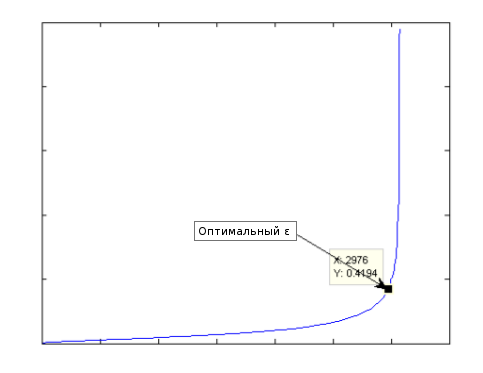
\includegraphics[width=\linewidth]{images/graph1.png}
  \caption{Кривая k-расстояний для одного уровня плотности}\label{fig:graph1}
\endminipage\hfill
\minipage{0.49\textwidth}%
  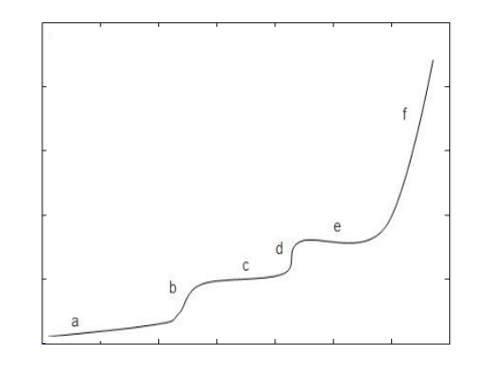
\includegraphics[width=\linewidth]{images/graph3.png}
  \caption{Кривая k-расстояний для нескольких уровней плотности}\label{fig:graph3}
\endminipage
}
\end{figure}
На графиках горизонтальные участки соответствуют уровням плотности в данных, вертикальные участки соответствуют уровням шумовых точек. Для определения оптимальных значений используются точки перемены знака второй производной графика, которая вычисляется по стандартной разностной схеме. 


\subsection{Процедуры корректного голосования}

Пусть H -- набор из r различных признаков вида H=$\{x_{j_1},...,x_{j_r}\}, \sigma=(\sigma_1,…,\sigma_r)$, $\sigma_i$ -- допустимое значение признака $x_{j_i}\text{, } i=\{1,...,r\}$. Пара $(\sigma,H)$ называется \textit{элементарным классификатором (эл.кл.)}.

Будем говорить, что объект $S \in M\text{, } S=\left(a_{1}, \ldots, a_{n}\right)$ \textit{содержит} эл.кл. $(\sigma, H)$, если $a_{j_{1}}=\sigma_{1}, \ldots, a_{j_{r}}=$ $\sigma_{r}$.

Величину $B(\sigma, S, H)$, равную 1 , если $S$ содержит эл.кл. $(\sigma, H)$, и 0 иначе, будем называть \textit{близостью объекта} $S$ к эл.кл. $(\sigma, H)$. 

Эл.кл. $(\sigma,H)$ называется \textit{корректным} для класса $K$, если не существует обучающих объектов $S^\prime$ и $S^{\prime\prime}$ таких, что $S^\prime \in K$, $S^{\prime\prime} \in \overline{K}$  и $B(\sigma, S^\prime, H)$ = $B(\sigma, S^{\prime\prime}, H)$ = 1.

Эл.кл. $(\sigma, H)$ называется \textit{представительным} для класса $K$, если ни один обучающий объект из $\overline{K}$ не содержит $(\sigma, H)$ и хотя бы один объект из $K$ содержит $(\sigma, H)$.

Представительный для класса $K$ эл.кл. называется \textit{тупиковым}, если не является представительным для $\overline{K}$ любой эл.кл. вида $(\sigma^\prime, H^\prime)$, где $\sigma^\prime=(\sigma_1,…,\sigma_{t-1},\sigma_{t+1},...,\sigma_r)\text{, }$ $H^\prime= H \setminus \{x_t\}, t \in \{1,2,...,r\}$.

Рассмотренные выше понятия могут быть введены с использованием аппарата нормальных форм булевых функций.

В случае бинарных данных нетрудно видеть, что эл.кл. $(\sigma, H)$, $H=\{x_{j_1},...,x_{j_r}\}, \sigma=(\sigma_1,…,\sigma_r)$, – это элементарная конъюнкция (ЭК) над переменными $x_1,…,x_n$ вида $x_{j_1}^{\sigma_1}...x_{j_r}^{\sigma_r}$, которая обращается в 1 на описании объекта S, если объект S содержит эл.кл. $(\sigma, H)$.

Представительный эл.кл. класса $K$ -- это ЭК, обращающаяся в 0 на всех прецедентах не из класса $K$ и обращающаяся в 1 хотя бы на одном прецеденте из класса $K$.

На этапе обучения для каждого класса $K$ строится свое множество тупиковых представительных эл.кл. $\cal T(\text{$K$})$. Построение таких множеств сводится к задаче монотонной дуализации - построению сокращенной дизъюнктивной нормальной формы монотонной булевой функции от n переменных, заданной конъюнктивной нормальной формой из |R| элементарных дизъюнкций. Существует также матричная формулировка задачи дуализации: поиск неприводимых покрытий булевой матрицы из |R| строк и n столбцов. Это труднорешаемая дискретная задача, в которой число решений растет экспоненциально с ростом числа переменных, поэтому для ее решения нужны эффективные алгоритмы. Наиболее эффективными считаются алгоритмы с полиномиальными задержками, но их удалось построить только для частных случаев монотонной дуализации. В 1977 г. Е. В. Дюковой был предложен подход к построению асимптотически оптимальных алгоритмов дуализации (алгоритмов, эффективных в «среднем»). На данный момент они являются лидерами по скорости счета. Примеры таких алгоритмов: АО1 и АО2 \cite{author7}, а также RUNC-M \cite{author12} и RUNC-M+ \cite{author9}.

Классификация объекта S осуществляется на основе процедуры голосования. Для этого вычисляется величина 
    $$\Gamma(S,K) =  \frac{1}{|\cal T(\text{K})|}\Sigma_{(\sigma, H) \in \cal T(\text{K})} P_{(\sigma, H)} B(\sigma,S,H)\text{,}$$

где $\cal T(\text{$K$})$ -- множество тупиковых представительных эл.кл. класса $K$, а $P_{(\sigma, H)}$ -- вес эл.кл. $(\sigma, H)$, то есть его информативность (например, число содержащих его прецедентов).

Объект $S$ относится к классу с максимальной оценкой. Если таких классов несколько, то происходит отказ от классификации объекта $S$.


\subsection{Восстановление значений целевой переменной}
После этапа кластеризации применяется алгоритм RUNC-M для решения возникшей задачи классификации. В процессе распознавания нового объекта сначала ему ставится метка кластера, к которому объект, вероятнее всего, относится. Далее определяется значение целевой переменной объекта, основываясь на значениях «ответа» объектов с соответствующей меткой кластера. Возможны различные подходы, например, использование среднего значения или медианы всех значений целевой переменной внутри класса. В данной работе применяется взвешенное усреднение по объектам того же кластера. В отличие от простого усреднения, значения целевой переменной учитываются с весами, обратно пропорциональными расстоянию (например, Евклидову расстоянию) до распознаваемого объекта \cite{author1_year}:\\

    $$\hat{y} = \sum_{i=1}^{n_k} w_iy_k^i\text{,}$$\\
    
    где $n_k$ -- число объектов в кластере $k$, $w_i = \frac{1}{d(x, x_i)}$ -- вес i-го объекта кластера $k$, $y_k^i$ -- «ответ»  i-го объекта кластера $k$.

\section{Вычислительные эксперименты}
В ходе проведения экспериментов, предложенный алгоритм (A1-Rg) был применен и анализировался на реальных данных из ресурса UCI: датасетах «Automobile», «Computer Hardware», «Servo», «Yacht Hydrodynamics» (источник - https://archive.ics.uci.edu). Цель экспериментов заключалась в сравнении полученных с помощью этого алгоритма результатов работы регрессионной модели с результатами, полученными при использовании классических методов восстановления регрессии.

Классические методы включали в себя: линейную регрессию (LR), регрессию методом k ближайших соседей (kNN-регрессия или kNR), градиентный бустинг (GB), регрессию с помощью метода опорных векторов (SVR) и алгоритм случайного леса (RF). Реализации используемых моделей была взята из библиотеки машинного обучения scikit-learn языка Python.

Перед началом эксперимента проводилась предобработка данных: вещественные признаки кодировались в категориальные путем разбиения на интервалы значений. Колонки с большим количеством уникальных значений удалялись. Объекты с пропущенными значениями также удалялись из выборки. Категориальные признаки кодировались в числовые значения.

Модели обучались и тестировались с использованием кросс-валидации. Данные разбивались на 5 фолдов, и один из фолдов откладывался для тестирования, в то время как остальные использовались для обучения. Процесс повторялся для каждого из 5 фолдов. Качество каждой модели оценивалось с помощью двух метрик: RMSE (Root Mean Squared Error - квадратный корень среднеквадратичной ошибки) и коэффициента детерминации R2: 

$$
RMSE = \sqrt{\frac{1}{n} \sum_{i=1}^{n}\left(y_{i}-\hat{y}_{i}\right)^{2}},
$$

\[R2 = 1 - \frac{\Sigma_{i=1}^{n}(y_i -\hat{y}_i)^{2}}{\Sigma_{i=1}^{n}(y_i - \bar{y})^{2}} \text{,} \]

где $y$ -- вектор истинных ответов для объектов тестовой выборки, $\hat{y}$ -- вектор предсказанных моделью ответов, \(\bar{y}\) — среднее значение вектора ответов.

Для получения более точной оценки моделей проводилось 10 независимых запусков на случайных разбиениях выборки на обучающую и тестовую. Результаты приведены в таблицах ниже.

\begin{table}[H]
\caption{Качество (RMSE)}
\begin{center}
\begin{tabular}{|c|c|c|c|c|c|c|}
    \hline
    Данные & LR & GB & kNR & RF & SVR & A1-Rg \\
    \hline
    Automobile (201 × 12) & 4221.20 & $\mathbf{2481.63}$ & 4291.69 & 2750.41 & 6601.70 & 6522.77  \\
    \hline
    Computer Hardware (209 × 9)  & 90.55 & $\mathbf{61.87}$ & 131.72 & 65.22 & 104.78 & 152.86  \\
    \hline
    Servo Data (167 × 6) & 1.15 & $\mathbf{0.45}$ & 0.91 & 0.49 & 0.66 & 1.34 \\
    \hline
    Yacht Hydrodyn. (308 × 7) & 9.37 & 5.76 & 7.55 & $\mathbf{4.91}$ & 6.42 & 8.99 \\
    \hline
\end{tabular}
\end{center}
\end{table}


\begin{table}[H]
\caption{Качество (R2 Score)}
\begin{center}
\begin{tabular}{|c|c|c|c|c|c|c|}
    \hline
    Данные & LR & GB & kNR & RF & SVR & A1-Rg \\
    \hline
    Automobile (201 × 12) & 0.73 & $\mathbf{0.90}$ & 0.71 & 0.88 & 0.35 & 0.36 \\
    \hline
    Computer Hardware (209 × 9) & 0.69 & $\mathbf{0.86}$ & 0.38 & 0.85 & 0.62 &  0.19 \\
    \hline
    Servo Data (167 × 6) & 0.45 & $\mathbf{0.91}$ & 0.66 & 0.90 & 0.81 & 0.27 \\
    \hline
    Yacht Hydrodyn. (308 × 7) & 0.63 & 0.86 & 0.76 & $\mathbf{0.90}$   & 0.83 & 0.66 \\
    \hline
\end{tabular}
\end{center}
\end{table}

Датасет "Automobile"(размер обучающей выборки: 201 объект × 12 признаков) включает в себя информацию об автомобилях, включая их технические характеристики, стоимость и другие свойства. На нем классические алгоритмы регрессии превосходят по качеству алгоритм A1-Rg значительно. Самыми эффективными являются GB и RF, которые обеспечивают наилучшую погрешность прогноза (RMSE) и коэффициент детерминации (R2 Score) соответственно. Тем не менее, быстрее всех работает kNR.


Задача "Computer Hardware" (размер обучающей выборки: 209 объектов × 9 признаков) включает в себя технические характеристики различных компонентов компьютера и их производительность. Здесь результат остается похожим: GB и RF показывают самую высокую точность среди классических методов, в то время как наименьшее время на вычисления уходит у kNR. Алгоритм A1-Rg вновь показывает себя хуже по всем показателям, включая время выполнения.

Задача "Servo" (размер обучающей выборки: 167 объектов × 6 признаков) представляет собой данные о работе сервопривода, включая такие параметры, как температура, вибрация, время отклика и др. GB отмечается превосходит остальные алгоритмы по обеим метрикам. В то же время, быстрее всего работает kNR.
A1-Rg уступает классическим методам, показывая более низкие значения метрик и более длительное время выполнения.

Задача "Yacht Hydrodynamics" (размер обучающей выборки: 308 объектов × 7 признаков). Этот датасет представляет собой данные о гидродинамических характеристиках яхт различных моделей и их свойствах. RF выделяется наилучшими показателями по обоим метрикам, однако, по времени работы он уступает LR.
A1-Rg сравним по качеству с классическими методами, но так же требует больше времени на обработку данных.

Подводя итог экспериментов, ансамблирующие методы в задаче регрессии, такие как GB и RF, показали более высокое качество распознавания по сравнению с алгоритмом A1-Rg на всех рассмотренных наборах данных.

\section{Использование логического корректора}
Ранее была реализована аналогичная композиция, которая базируется на логических корректорах в качестве распознающих процедур. В алгебраическом подходе несколько распознающих алгоритмов объединяются в один для взаимной коррекции ошибок. Логические корректоры, хорошо зарекомендовавшие себя при решении прикладных задач, базируются на построении корректных наборов из произвольных элементарных классификаторов. В \cite{lyubimtseva14} разработан стохастический вариант логического корректора MONS. Его применение в регрессионной модели на этапе после сведения к задаче классификации по прецедентам позволило улучшить качество распознавания на тех же задачах в сравнеии с классическими алгоритмами регрессии:

\begin{table}[H]
\caption{Качество (MSE)}
\begin{center}
\begin{tabular}{|c|c|c|c|c|c|}
\hline
Данные & MONS-Rg & LR & kNN & GB \\
\hline
Servo               & 0.95662 & 1.37443  & 0.94863 & $\mathbf{0.18757}$\\
Computer Hardware  & $\mathbf{3908.57}$ & 8128.60 & 8409.37 & 4285.30\\
Yachts Hydrodyn.              & 248.166 & 85.5714 & 137.483 & $\mathbf{0.64404}$\\

\hline
\end{tabular}
\end{center}
\end{table}

\section{Модификация предложенного подхода}
Так, определено дальнейшее направление работы:
\begin{itemize}
  \item строить голосование над элементарными классификаторами, стараясь оптимизировать потери для задачи регрессии
  \item использовать ансамблирование: бэггинг или бустинг. Ниже описан вариант реализации обучения бустинга.
\end{itemize}

\begin{algorithm}[H]
\SetAlgoLined
\SetKwInOut{Input}{Вход}
\SetKwInOut{Output}{Выход}
\SetKw{Return}{вернуть}
\SetKw{In}{в}
\Input{Набор данных $S$, количество итераций $T$}
\Output{Композиция алгоритмов $\{h_t\}_{t=1}^{T}$}
\BlankLine
Инициализация $r_i \leftarrow y_i - \frac{1}{|S|}\sum_{i=1}^{|S|}y_i$ для всех $i \in \{1, \ldots, |S|\}$\;
\For{$t \leftarrow 1$ \KwTo $T$}{
  Выбираем объект с наибольшим остатком $r_i$\;
  $S_{i_t} = \{\tilde{S}_i\}_{i=1}^{r}$\;
  Построение булевой матрицы сравнения $L_t$\;
  \For{$i \leftarrow 1$ \KwTo $r$}{
   \For{$j \leftarrow 1$ \KwTo $n$}{
  $a_{ij} \leftarrow \left[x_j(S_{k_i}) \neq x_j(S_{i_t})\right]$\;
 }
  }
  $h_t \leftarrow \text{обучаем базовый алгоритм, используя } L_t$\;
  Вычисляем оптимальный вес $\alpha_t$\;
  Обновляем остатки $r_i$\;
}
\Return{$\{h_t\}_{t=1}^T$}
\caption{Псевдокод алгоритма бустинга}
\end{algorithm}

\begin{figure}[H]
\noindent\centering{
{\textwidth}
  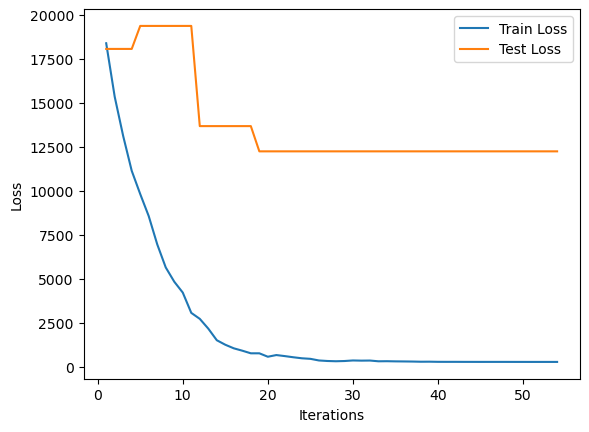
\includegraphics[width=\linewidth]{images/boosting_loss_1.png}
  \caption{Поведение лосса при обучении и тестировании модели бустинга на игрушечных данных}\label{fig:graph1}
\hfill
}
\end{figure}
Из графика видно, что потери во время обучении выходят на плато, а на тестовой выборке модель не выдала приемлемое качество в силу использования только отношения неравенства на множестве значений признаковых описаний объектов и ограниченности разнообразия примеров: использовался игрушечный набор данных, содержащий 50 объектов. Как следствие, модель переобучается и отказывается распознавать новые объекты на определенном этапе. В дальнейшем необходимо использовать отношения порядка на множестве значений признаков для выделения более сложных логических закономерностей и уменьшения отказов в распознавании.

\section{Заключение}

В настоящей работе предложен метод, решающий задачу сведением к классификации по прецедентам на основе логического подхода. Разработан алгоритм A1-Rg, состоящий из следующих этапов: кластеризация данных, классификация по тупиковым представительным эл.кл. и восстановление регрессии на основе взвешенного усреднения. Полученные результаты показали, что алгоритм A1-Rg не достигает достаточной эффективности в плане качества предсказаний по сравнению с классическими алгоритмами. Приведены результаты тестирования алгоритма, основанного на использовании стохастической модификации логического корректора (алгоритм MONS), на прикладных задачах. Поставленная задача решена путем использования ансамбля алгоритмов.



% \section{Headings: first level}
% \label{sec:headings}

% \lipsum[4] See Section \ref{sec:headings}.

% \subsection{Headings: second level}
% \lipsum[5]
% \begin{equation}
% 	\xi _{ij}(t)=P(x_{t}=i,x_{t+1}=j|y,v,w;\theta)= {\frac {\alpha _{i}(t)a^{w_t}_{ij}\beta _{j}(t+1)b^{v_{t+1}}_{j}(y_{t+1})}{\sum _{i=1}^{N} \sum _{j=1}^{N} \alpha _{i}(t)a^{w_t}_{ij}\beta _{j}(t+1)b^{v_{t+1}}_{j}(y_{t+1})}}
% \end{equation}

% \subsubsection{Headings: third level}
% \lipsum[6]

% \paragraph{Paragraph}
% \lipsum[7]



% \section{Examples of citations, figures, tables, references}
% \label{sec:others}

% \subsection{Citations}
% Citations use \verb+natbib+. The documentation may be found at
% \begin{center}
% 	\url{http://mirrors.ctan.org/macros/latex/contrib/natbib/natnotes.pdf}
% \end{center}

% Here is an example usage of the two main commands (\verb+citet+ and \verb+citep+): Some people thought a thing \citep{kour2014real, hadash2018estimate} but other people thought something else \citep{kour2014fast}. Many people have speculated that if we knew exactly why \citet{kour2014fast} thought this\dots

% \subsection{Figures}
% \lipsum[10]
% See Figure \ref{fig:fig1}. Here is how you add footnotes. \footnote{Sample of the first footnote.}
% \lipsum[11]

% \begin{figure}
% 	\centering
% 	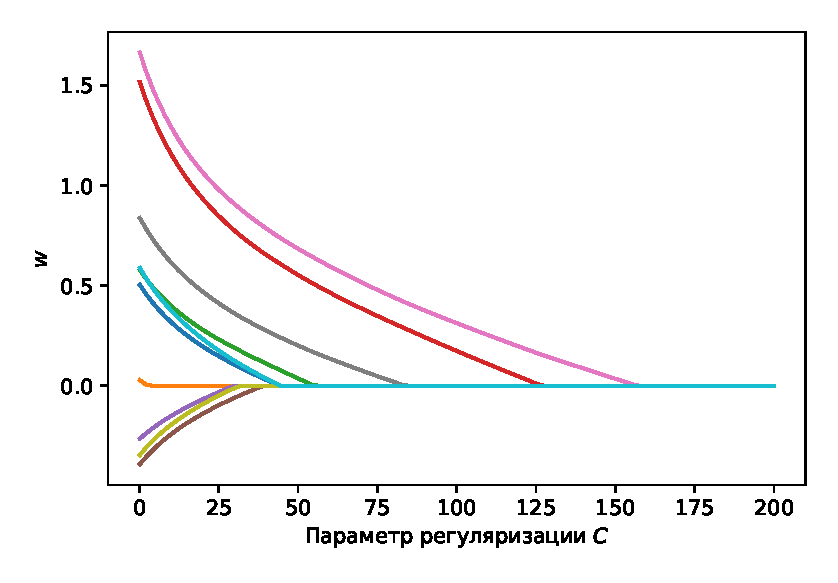
\includegraphics[width=0.5\textwidth]{../figures/log_reg_cs_exp.eps}
% 	\caption{Sample figure caption.}
% 	\label{fig:fig1}
% \end{figure}

% \subsection{Tables}
% See awesome Table~\ref{tab:table}.

% The documentation for \verb+booktabs+ (`Publication quality tables in LaTeX') is available from:
% \begin{center}
% 	\url{https://www.ctan.org/pkg/booktabs}
% \end{center}


% \begin{table}
% 	\caption{Sample table title}
% 	\centering
% 	\begin{tabular}{lll}
% 		\toprule
% 		\multicolumn{2}{c}{Part}                   \\
% 		\cmidrule(r){1-2}
% 		Name     & Description     & Size ($\mu$m) \\
% 		\midrule
% 		Dendrite & Input terminal  & $\sim$100     \\
% 		Axon     & Output terminal & $\sim$10      \\
% 		Soma     & Cell body       & up to $10^6$  \\
% 		\bottomrule
% 	\end{tabular}
% 	\label{tab:table}
% \end{table}

% \subsection{Lists}
% \begin{itemize}
% 	\item Lorem ipsum dolor sit amet
% 	\item consectetur adipiscing elit.
% 	\item Aliquam dignissim blandit est, in dictum tortor gravida eget. In ac rutrum magna.
% \end{itemize}


\bibliographystyle{plainnat}
\bibliography{references}

\end{document}
